\documentclass{standalone}
\usepackage{tikz}
\usepackage{bm}
\usepackage{amsmath}
\usepackage{xcolor}

\begin{document}
    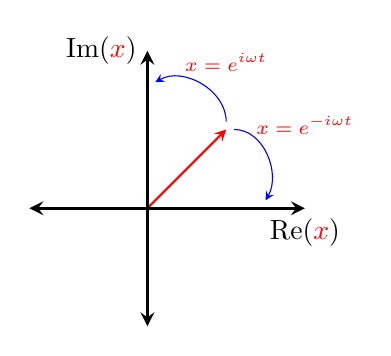
\begin{tikzpicture}
    
        % Phasor arrow
        \draw[->, thick, red, >=stealth] (0,0) -- (1,1) node[left] {};
        
        % Axes
        \draw[<->, very thick, >=stealth] (-1.5,0) -- (2,0) node[below] {$\operatorname{Re}(\textcolor{red}{x})$};
        \draw[<->, very thick, >=stealth] (0,-1.5) -- (0,2) node[left] {$\operatorname{Im}(\textcolor{red}{x})$};

        % Rotation arrow labels
        \node[red] at (1.0,1.85) {\scriptsize $x=e^{i\omega t}$};
        \node[red] at (2,1.05) {\scriptsize $x=e^{-i\omega t}$};
        
        % Rotations
        \draw [->,blue, >=stealth] (1.0,1.1) to [out=90,in=30] (0.1,1.6);
        \draw [->,blue, >=stealth] (1.1,1) to [out=0,in=60] (1.5,0.1);
        
    \end{tikzpicture}
\end{document}